\documentclass[11pt,twoside]{article}

% Text
\usepackage[utf8]{inputenc}

% Graphics
\usepackage{graphicx}
\usepackage{graphics}
\usepackage[dvipsnames, table]{xcolor}
\usepackage{tikz}
\usepackage{microtype}
\usepackage{setspace}

% Geometry
\usepackage{geometry}
 \geometry{
 a4paper,
 left=25mm,
 right=25mm,
 top=30mm,
 bottom=25mm,
 heightrounded,
 headsep=7mm}

% URL
\usepackage{hyperref}

% Tables
\usepackage{tabu}
\usepackage{tabularx}
\usepackage{ltablex}
\usepackage{longtable}
\usepackage{float}
\usepackage{makecell}
\usepackage{array}

\begin{document}

\begin{center}
\thispagestyle{empty}

\includegraphics[scale=1.25]{Images/PolimiLogo}\\
\vspace{4cm}
\textbf{\Huge{Design Document}}\\
\vspace{1.5cm}
\textbf{\Large{Version 1.0}}\\
\bigskip \par
by \par
\large{Abdallah Alkhetiar}\\
\large{Daniel Bonardi}\\
\bigskip \bigskip
\large{\today}
\end{center}

\newpage

\setcounter{page}{1}
\begin{center}
\textbf{\Huge{Document details}}
\end{center}
\begin{table}[h!]
\begin{tabu} to \textwidth { |X[0.25,r,p] || X[0.75,l,p]| }
\hline

\textbf{Deliverable:} & DD \\
\hline
\textbf{Title:} & Design Document \\
\hline
\textbf{Authors:} & Abdallah Alkhetiar and Daniel Bonardi \\
\hline
\textbf{Version:} & 1.0 \\ 
\hline
\textbf{Date:} & \today \\
\hline
\textbf{Download page:} & \href{https://github.com/Zero3474/AlkhetiarBonardi.git}{\texttt{\color{blue}{github.com/Zero3474/AlkhetiarBonardi.git}}} \\
\hline
\textbf{Copyright:} & Copyright © 2025, Abdallah Alkhetiar and Daniel Bonardi \\
& – All rights reserved \\
\hline
\end{tabu}
\end{table}

\newpage

\tableofcontents

\newpage

\section{Introduction}
	\subsection{Purpose}
This design document outlines the architectural framework, user interface design, and other system components necessary to meet the functional and non-functional requirements described in the Requirement Analysis and Specification Document. \\
It also serves as a foundation for developers, testers, and stakeholders to understand the system's structure and ensures that the final implementation adheres to the defined goals. \\
The main purpose of the S\&C platform is to grant efficient and effective matchmaking between university students seeking experience through internships and companies offering them. The design aims to ensure:
\begin{itemize}
\item \textbf{Precision in matching}: The system adopts a sophisticated recommendation system to notify students about suitable internships, based on criteria such as skills and experiences.
\item \textbf{Smooth user experience}: The system shall grant its users the best experience by smoothly managing all internship-related workflows, including searching, application, selection, feedback collection, and monitoring of ongoing internships.
\item \textbf{Scalability}: The system's design shall accommodate future adjustments, such as advanced data analytics, integration with external tools, or even an expanded scope.
\end{itemize}

	\subsection{Scope}
\textbf{Students\&Companies} (S\&C) is an internship platform designed to connect students with companies based on skills, experiences, and interests. \\
The platform offers two main ways to establish connections:
\begin{itemize}
\item \textbf{Recommendation system}
\item \textbf{Proactive searching}
\end{itemize}
S\&C also supports the selection process  and gathers feedback on recommendations and provides spaces for users to address issues, share updates, and track internship progress.
More details can be found in the RASD document.
	\subsection{Definitions, acronyms, abbreviations}
TBD

	\subsection{Revision history}
Version 1.0 - WIP

	\subsection{Reference documents}
TBD

	\subsection{Document structure}
\textbf{Section 1: Introduction} \\
This section is presented with a brief overview of this document's content including the description of the purpose, the scope, and all the definitions, acronyms and abbreviations used.
\vspace{1\baselineskip} \\
\textbf{Section 2: Architectural design} \\
This section is presented with a detailed description of the architectural choices for the system, including a high-level description of the system and its components. In addition it is presented a detailed description of the deployment view and the main runtime views of the system.
\vspace{1\baselineskip} \\
\textbf{Section 3: User interface design} \\
This section is presented with a series of prototypes for the most important pages of the software to help graphic designers. Each image is accurately described to avoid any misunderstanding on the pages' available functionalities.
\vspace{1\baselineskip} \\
\textbf{Section 4: Requirements traceability} \\
This section is highly dependent on the RASD, as it provides a complete mapping of both functional and non-functional requirements described in that document, with the modules introduced and described in this document.
\vspace{1\baselineskip} \\
\textbf{Section 5: Implementation, integration and test plan} \\
The last section describes the procedures followed for implementing, integrating and testing the components of the platform.

\newpage

\section{Architectural design}
	\subsection{Overview}	
The S\&C design is based on two architectural choices:
\begin{itemize}
\item A 3 tier architecture
\item A thin-client model
\end{itemize}
First of all the 3 tier architecture is built using 3 layers:
\begin{itemize}
\item \textbf{Presentation layer}: This layer is in charge of providing all the user interfaces for users to interact with the system.
\item \textbf{Application layer}: This layer implements the core of the business logic and processes all the requests sent from the presentation layer.
\item \textbf{Data layer}: This layer is responsible of managing all the data storage.
\end{itemize}
The choice of the 3 tier architecture what made to grant these key concepts:
\begin{itemize}
\item \textbf{Modularity}: Components are designed address a specific function required by the system, also making it easier to perform maintenance.
\item \textbf{Scalability}: Since each module function independently from the others, adding or removing feature should be easier.
\item \textbf{Security}: By implementing a secure communication protocol, users should not be worried about their sensitive data being stolen.
\end{itemize}
The thin-client approach instead, ensures the smoothest experience for the users, by keeping the client-side of the application as lightweight as possible. With this approach the client shall focus solely on the rendering of the user interface and the management of basic interactions, the rest of the computation happens on the server-side.\\
To sum it up, in the client there is only the presentation layer, while the application and data layer are in the server.

	\subsection{Component view}
To make it easier to understand component view, we decided to divide it into 3 diagrams. The first represents a high-level view that distinguishes the client-side from the server-side components. The other 2 diagrams represent a more detailed version of the components presented in the server-side in the first diagram.

		\subsubsection{High level component view}
In the following diagram it is shown how the client-side interacts with the server side through the exposed interfaces.\\
We can clearly see the 2 sides:
\begin{itemize}
\item \textbf{Client-side}: Since the in the client-side we only have the presentation layer, we can see that on the left of the diagram there are the Users, that can either be accessing the application through a web browser or a mobile device.
\item \textbf{Server-side}: On the server-side instead, we have both the application and data layer so we have the most important subsystems of the entire application:
	\begin{itemize}
	\item \textit{Internship management}: Which is the actual biggest component which manages all the actions that involve internships.
	\item \textit{Account management}: Which simply manages all the interactions that require some data regarding a user.
	\end{itemize}
\end{itemize}

\begin{figure}[H]
\centering
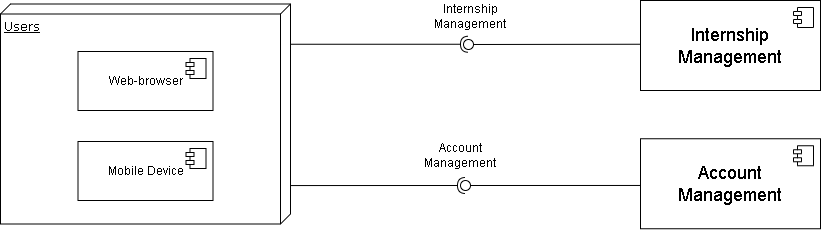
\includegraphics[width=0.9\textwidth]{Images/Component}
\caption{High level component view}\label{Component}
\end{figure}
\vspace{\baselineskip}

		\subsubsection{Internship management diagram}
The following diagram shows how the subsystem Internship Management is composed and how its modules communicate with external ones. This subsystem contains 6 modules:	
\begin{itemize}
\item \textbf{Proactive search}: Allows student to search for specific internship.
\item \textbf{Internship archival}: Allows companies to archive an internship, and show it on their profile.
\item \textbf{Feedback}: Allows user to send a feedback.
\item \textbf{Internship creation}: Allows companies to create an internship, and for this reason it needs to interact with the "Recommendation system" component to notify the compatible students.
\item \textbf{Complaints}: Allows user to file a complaint, and it also needs to interact with the "Notification system" to notify the universities.
\item \textbf{Form management}: Manages all the stages of a form, from its creation to the correction, and for this reason it needs to interact with the "Ranking system" component.
\end{itemize}
At the same time all components, external or internal to the subsystem, must interact with the DBMS to access all the data required for the interaction.
\newpage

\begin{figure}[H]
\centering
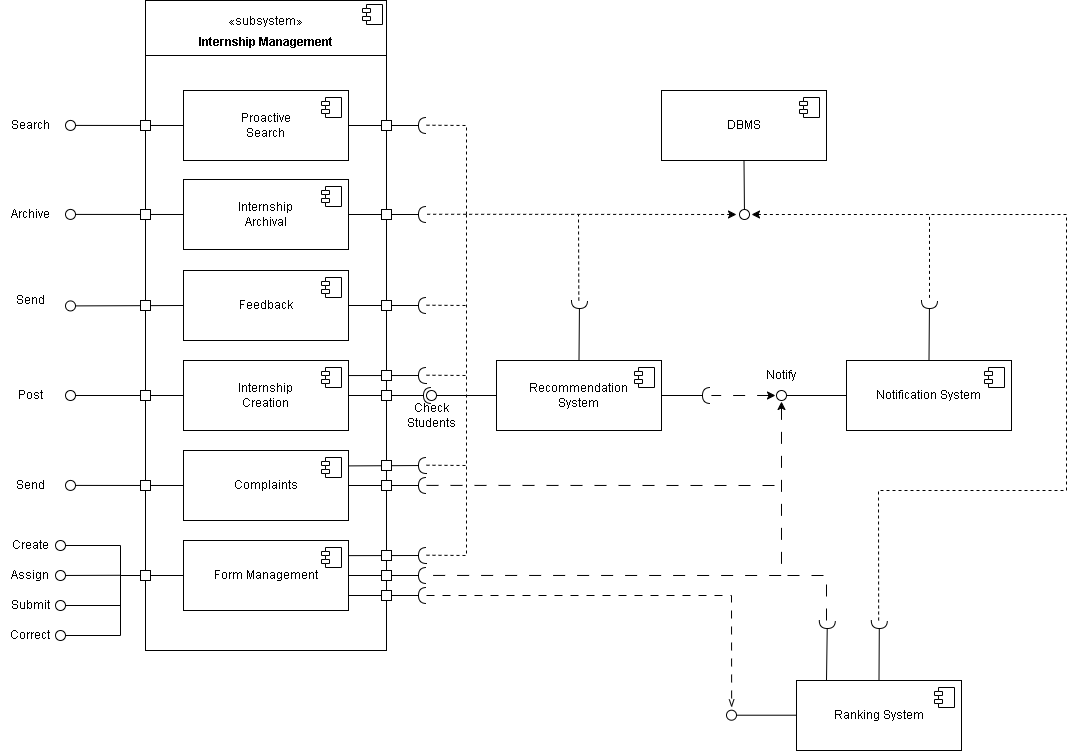
\includegraphics[width=0.95\textwidth]{Images/Component2}
\caption{Internship management diagram}\label{Component2}
\end{figure}
		
		\subsubsection{Account management diagram}
The following diagram shows how the subsystem Account Management is composed and how its modules communicate with external ones. This subsystem contains only 2 modules:
\begin{itemize}
\item \textbf{Student manager}: Allows student to sign up, login, add a CV and update their profile.
\item \textbf{Company manager}: Allows a company to sign up, login and update their profile.
\end{itemize}
In both cases the component need to access both the "Authentication" component to safely complete the login and sign up processes, and also the DBMS to manage all the required data.

\begin{figure}[H]
\centering
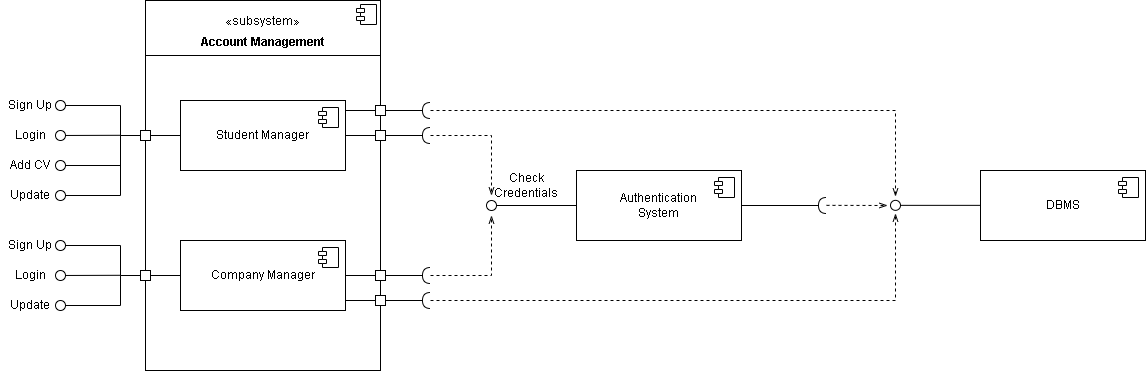
\includegraphics[width=0.95\textwidth]{Images/Component3}
\caption{Account management diagram}\label{Component3}
\end{figure}

\newpage

	\subsection{Deployment view}
 
	\subsection{Runtime view}
With the following sequence diagrams, we are going to explain and represent all the interactions that happen between the components of the S\&C system. But since this representation is still a high-level description of interactions, the function names, parameters, results, errors, and other smaller details will be modified or added during the development phase.

		\subsubsection{Login}
\begin{figure}[H]
\centering
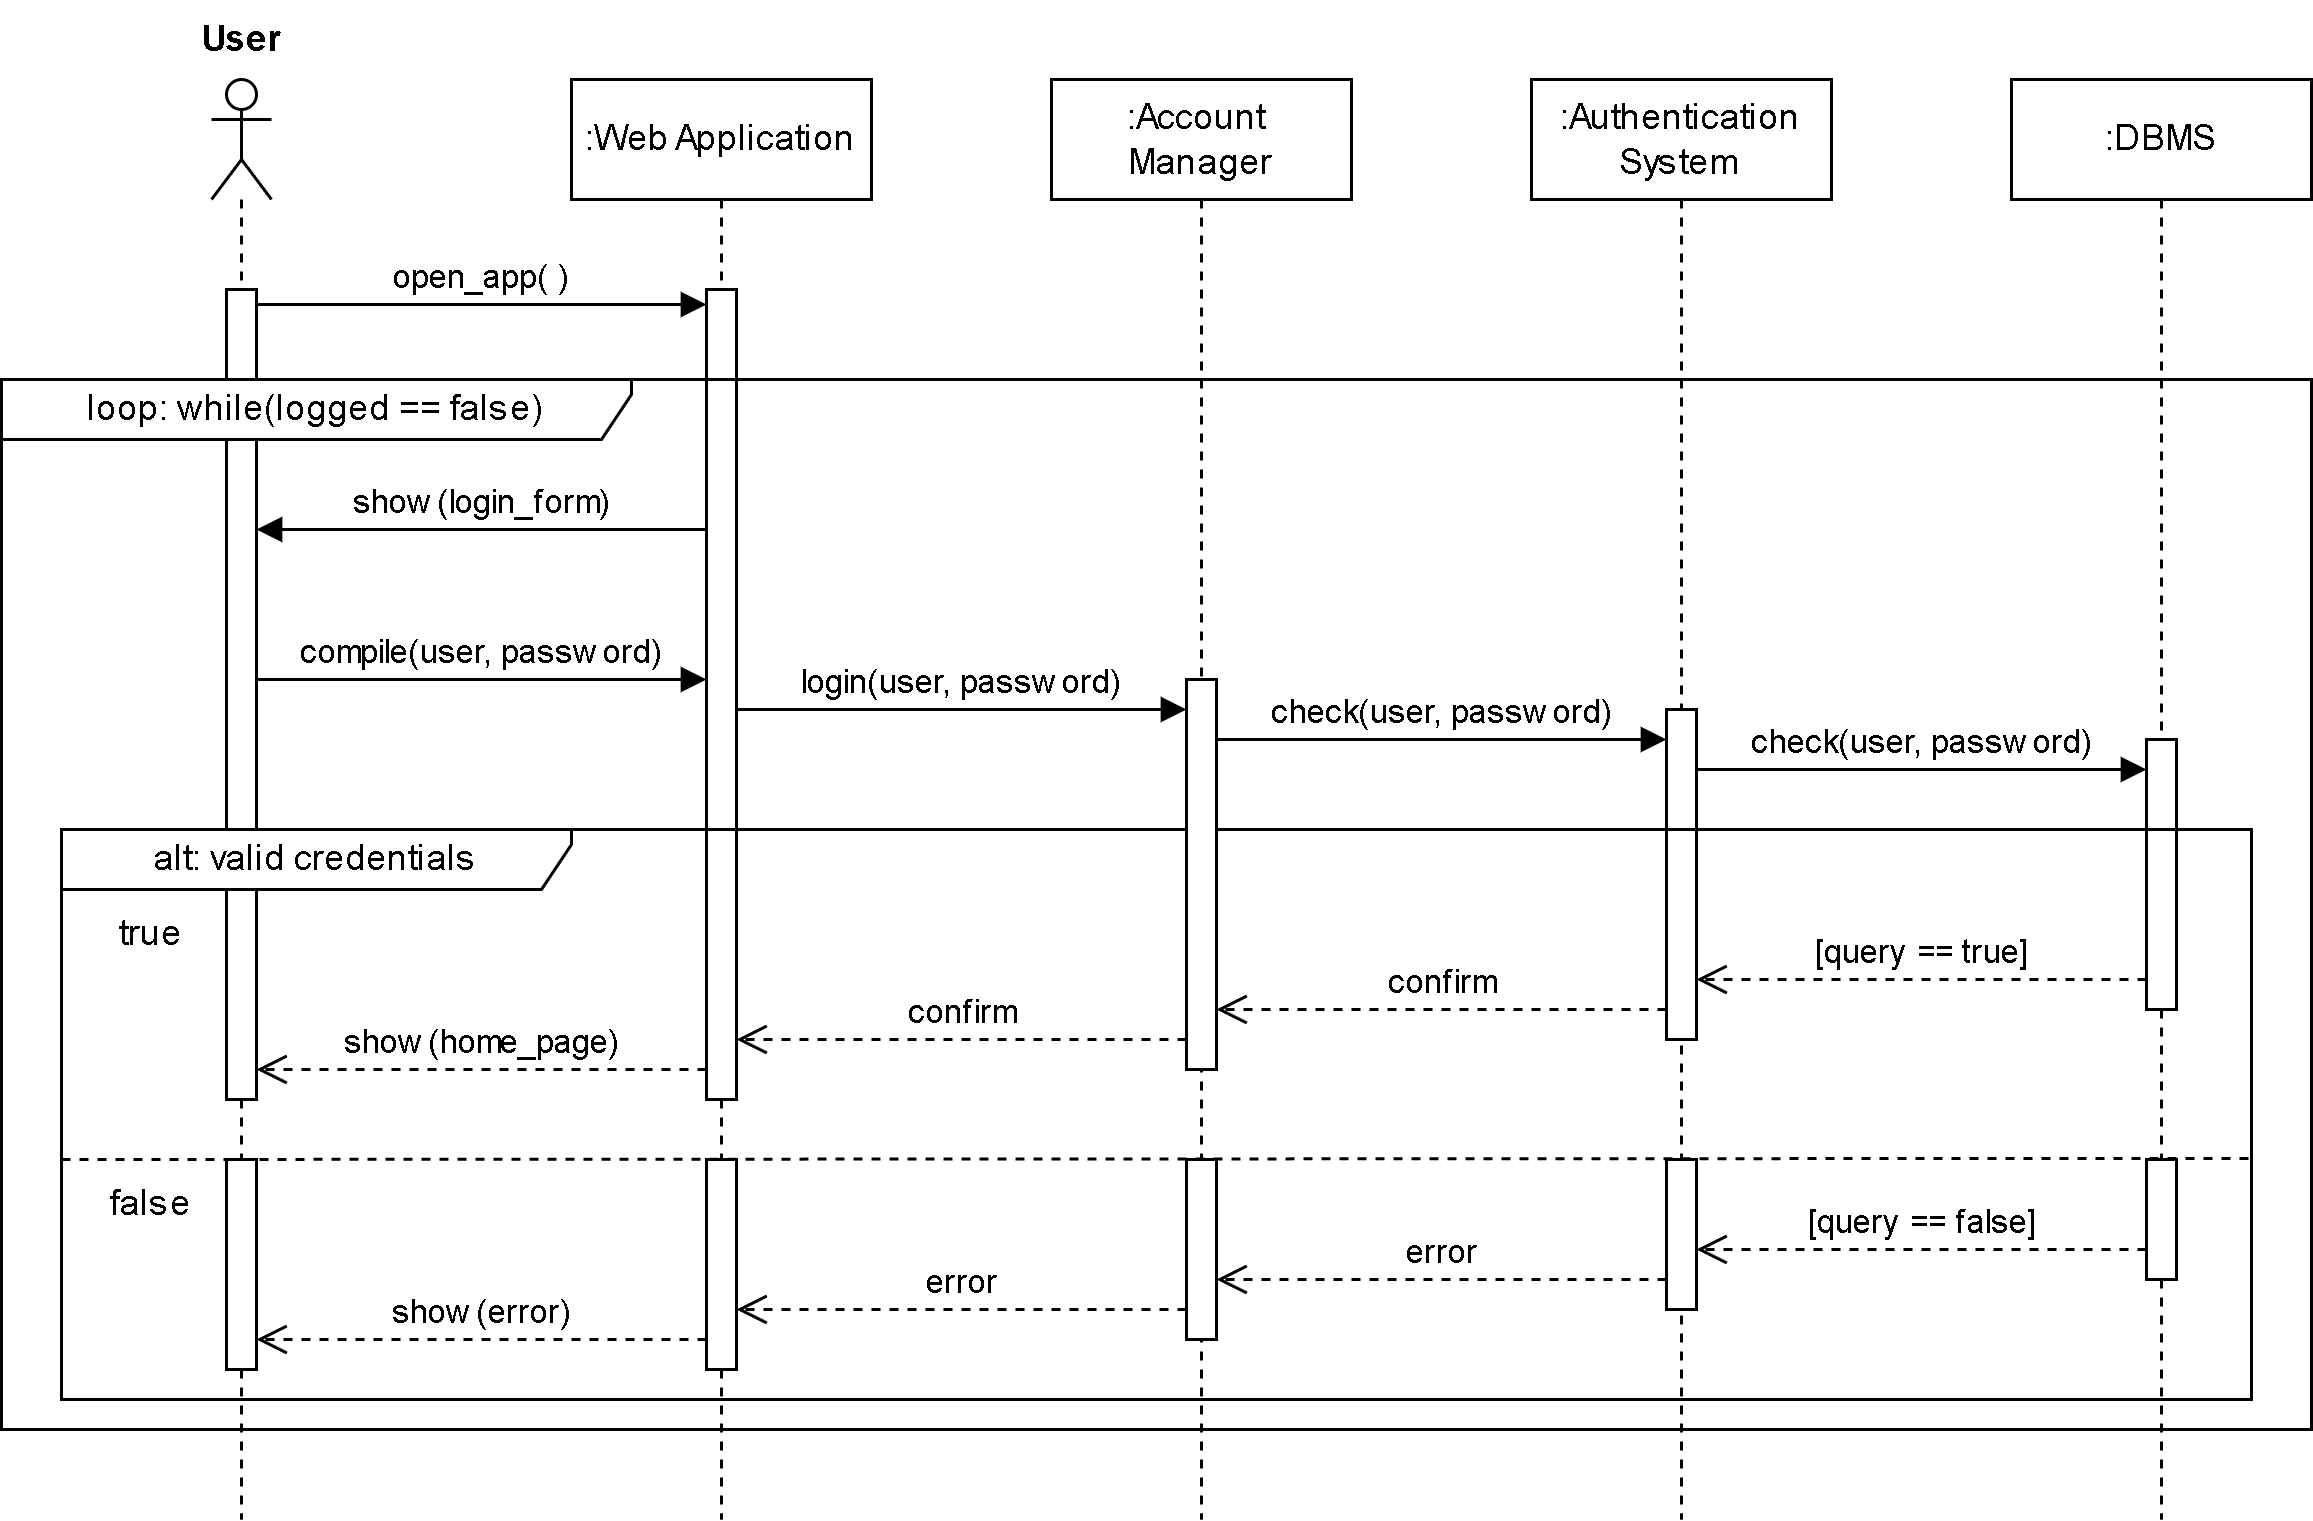
\includegraphics[width=0.95\textwidth]{Images/Seq1}
\caption{Login sequence diagram}\label{Seq1}
\end{figure}

\newpage

		\subsubsection{Sign up}
\begin{figure}[H]
\centering
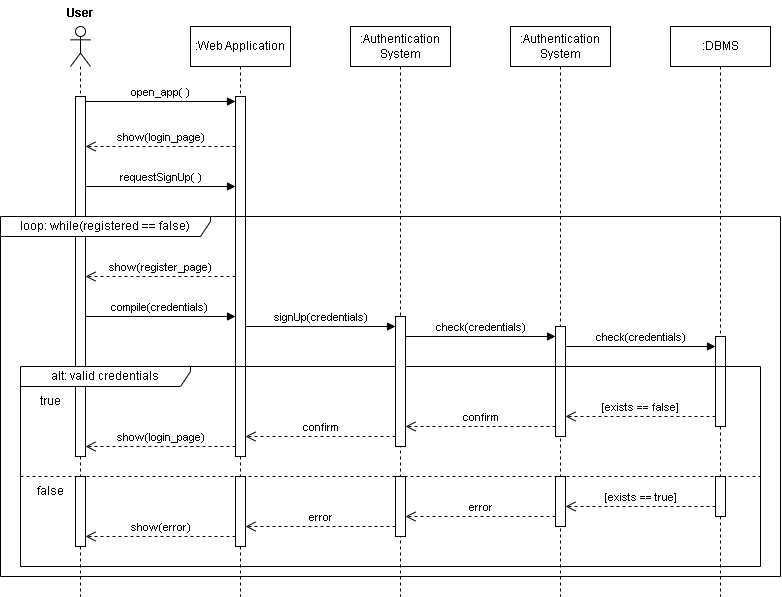
\includegraphics[width=0.95\textwidth]{Images/Seq2}
\caption{Sign up sequence diagram}\label{Seq2}
\end{figure}

\newpage

		\subsubsection{Internship creation}
\begin{figure}[H]
\centering
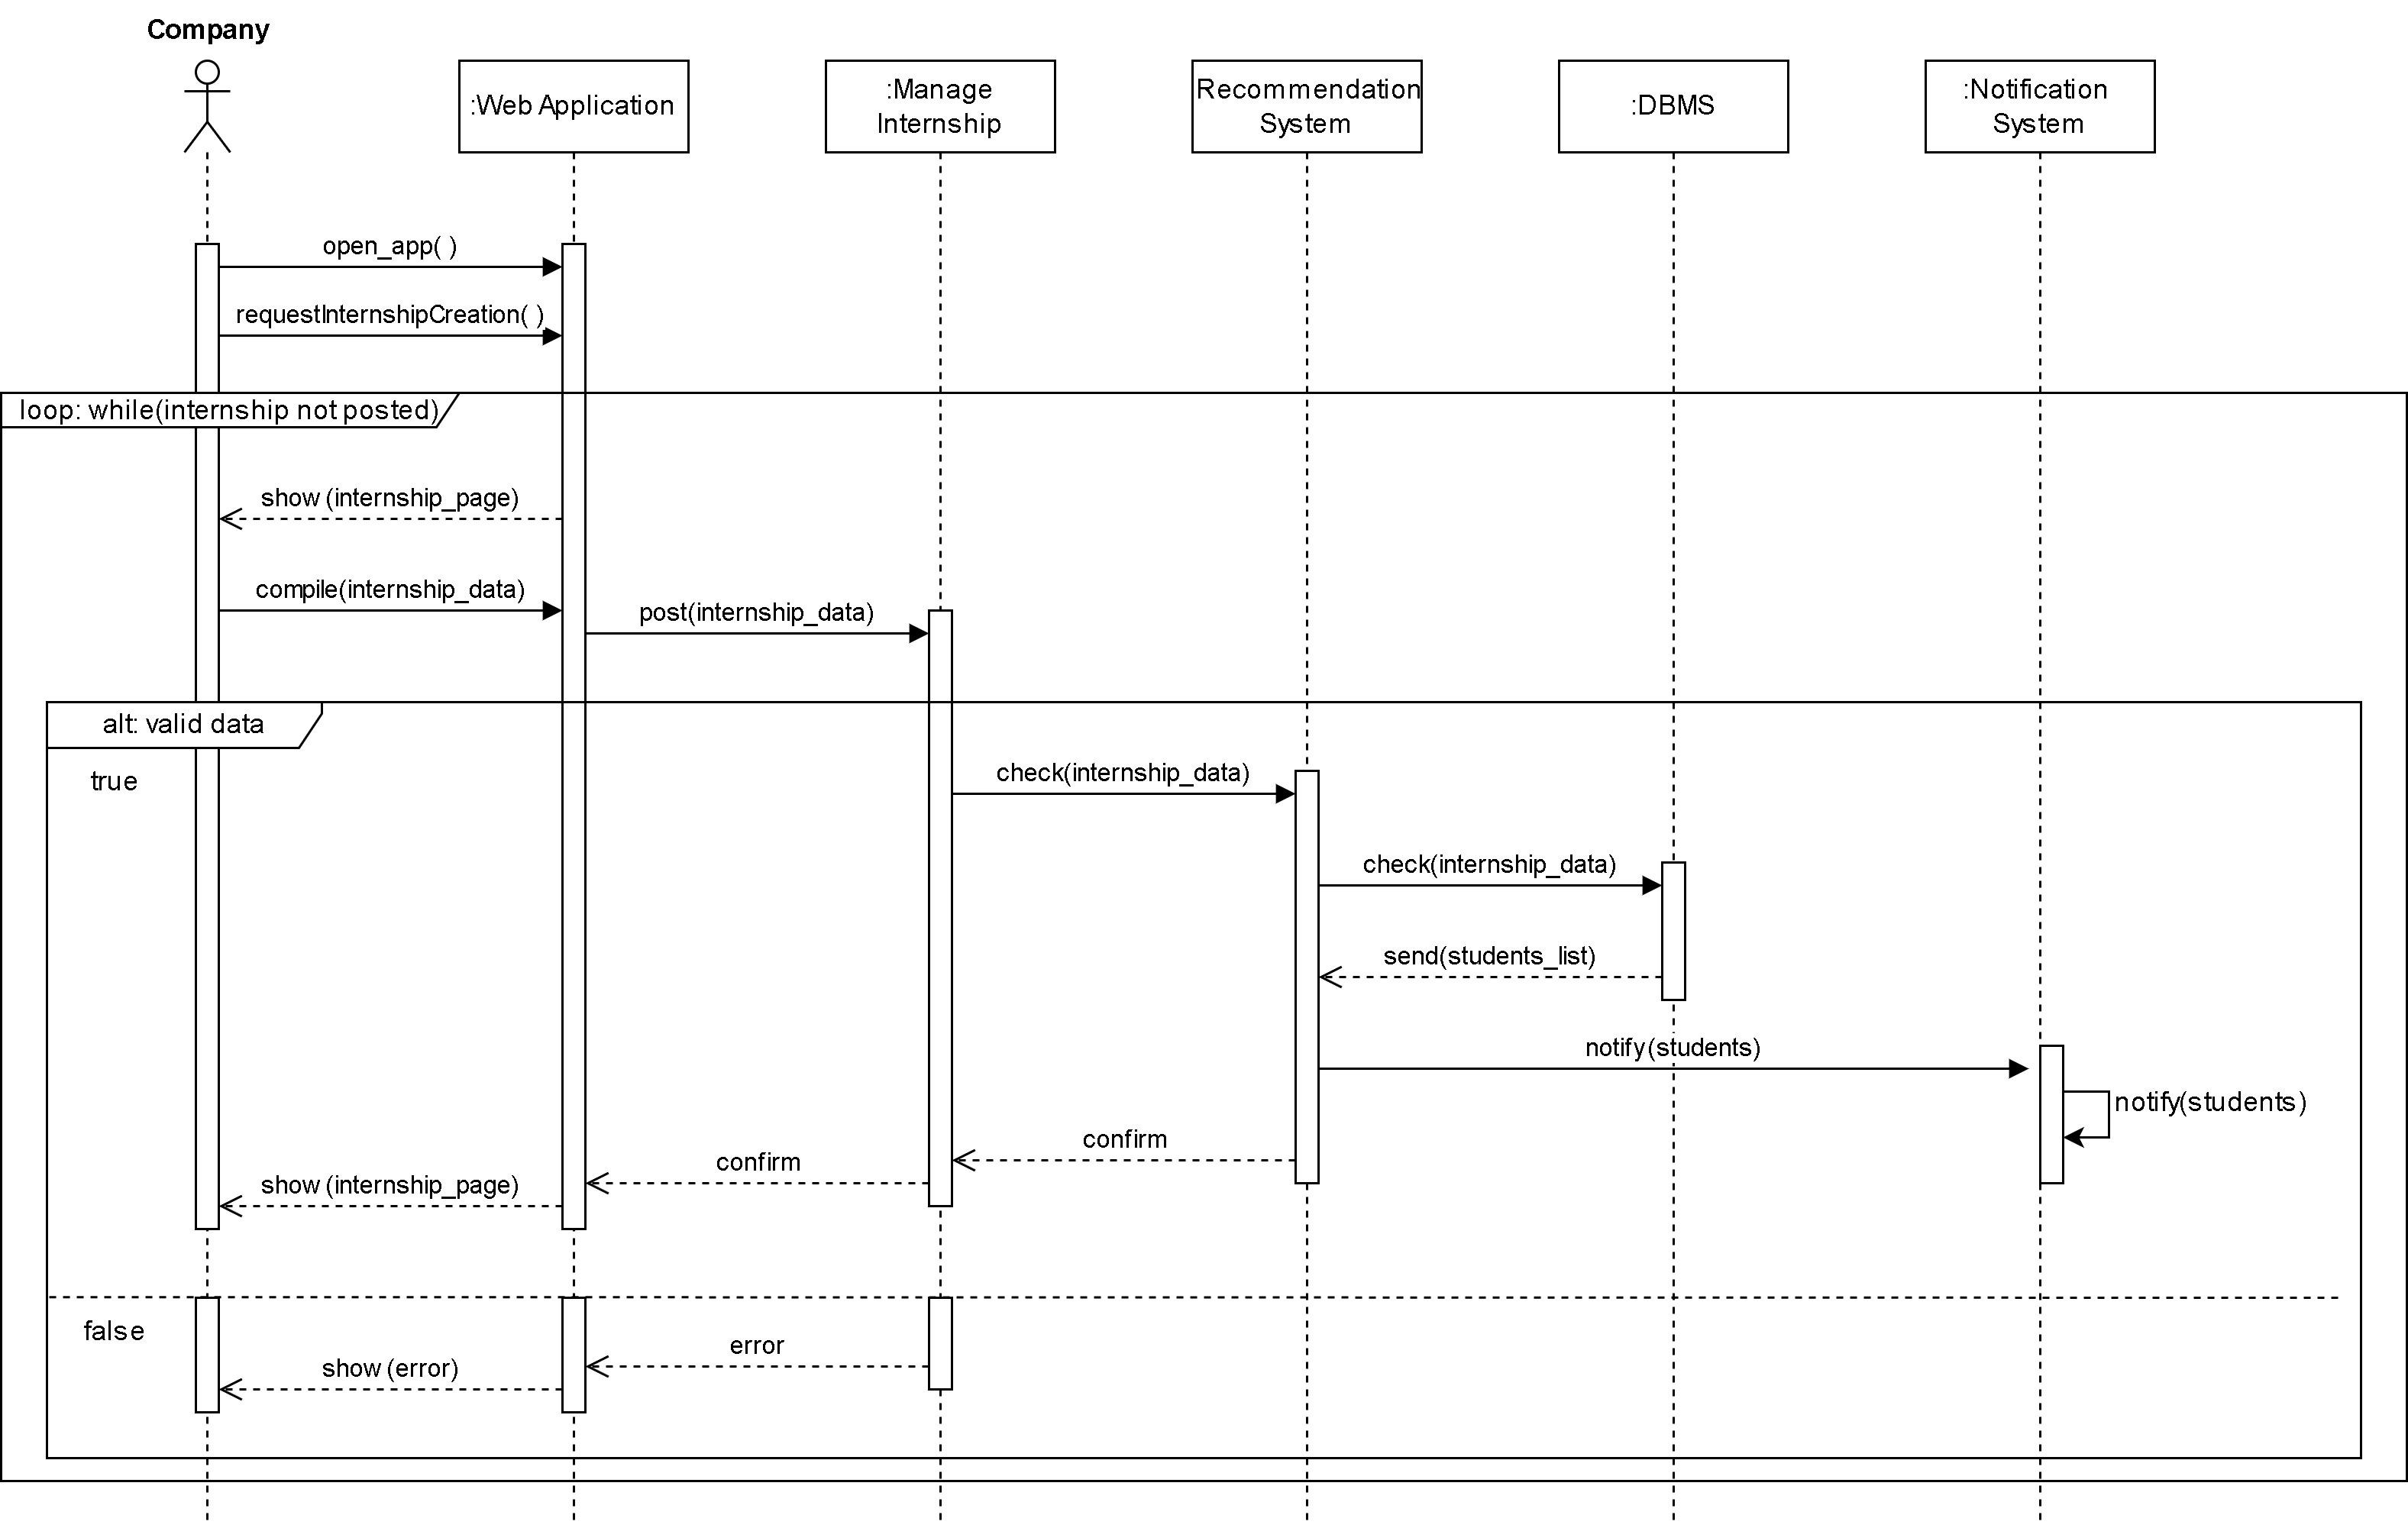
\includegraphics[width=0.95\textwidth]{Images/Seq3}
\caption{Internship creation sequence diagram}\label{Seq3}
\end{figure}

\newpage
	
	\subsection{Component interfaces}
	
	\subsection{Selected architectural styles and patterns}
	
	\subsection{Other design decisions}

\newpage

\section{User interface design}
The aim of this section is to present the prototypes of the most important pages of the application and explain the features by emulating scenarios of a user interacting with the system.
\vspace{1\baselineskip} \\
\large{\textbf{Login and Sign Up page}}
\begin{figure}[H]
\centering
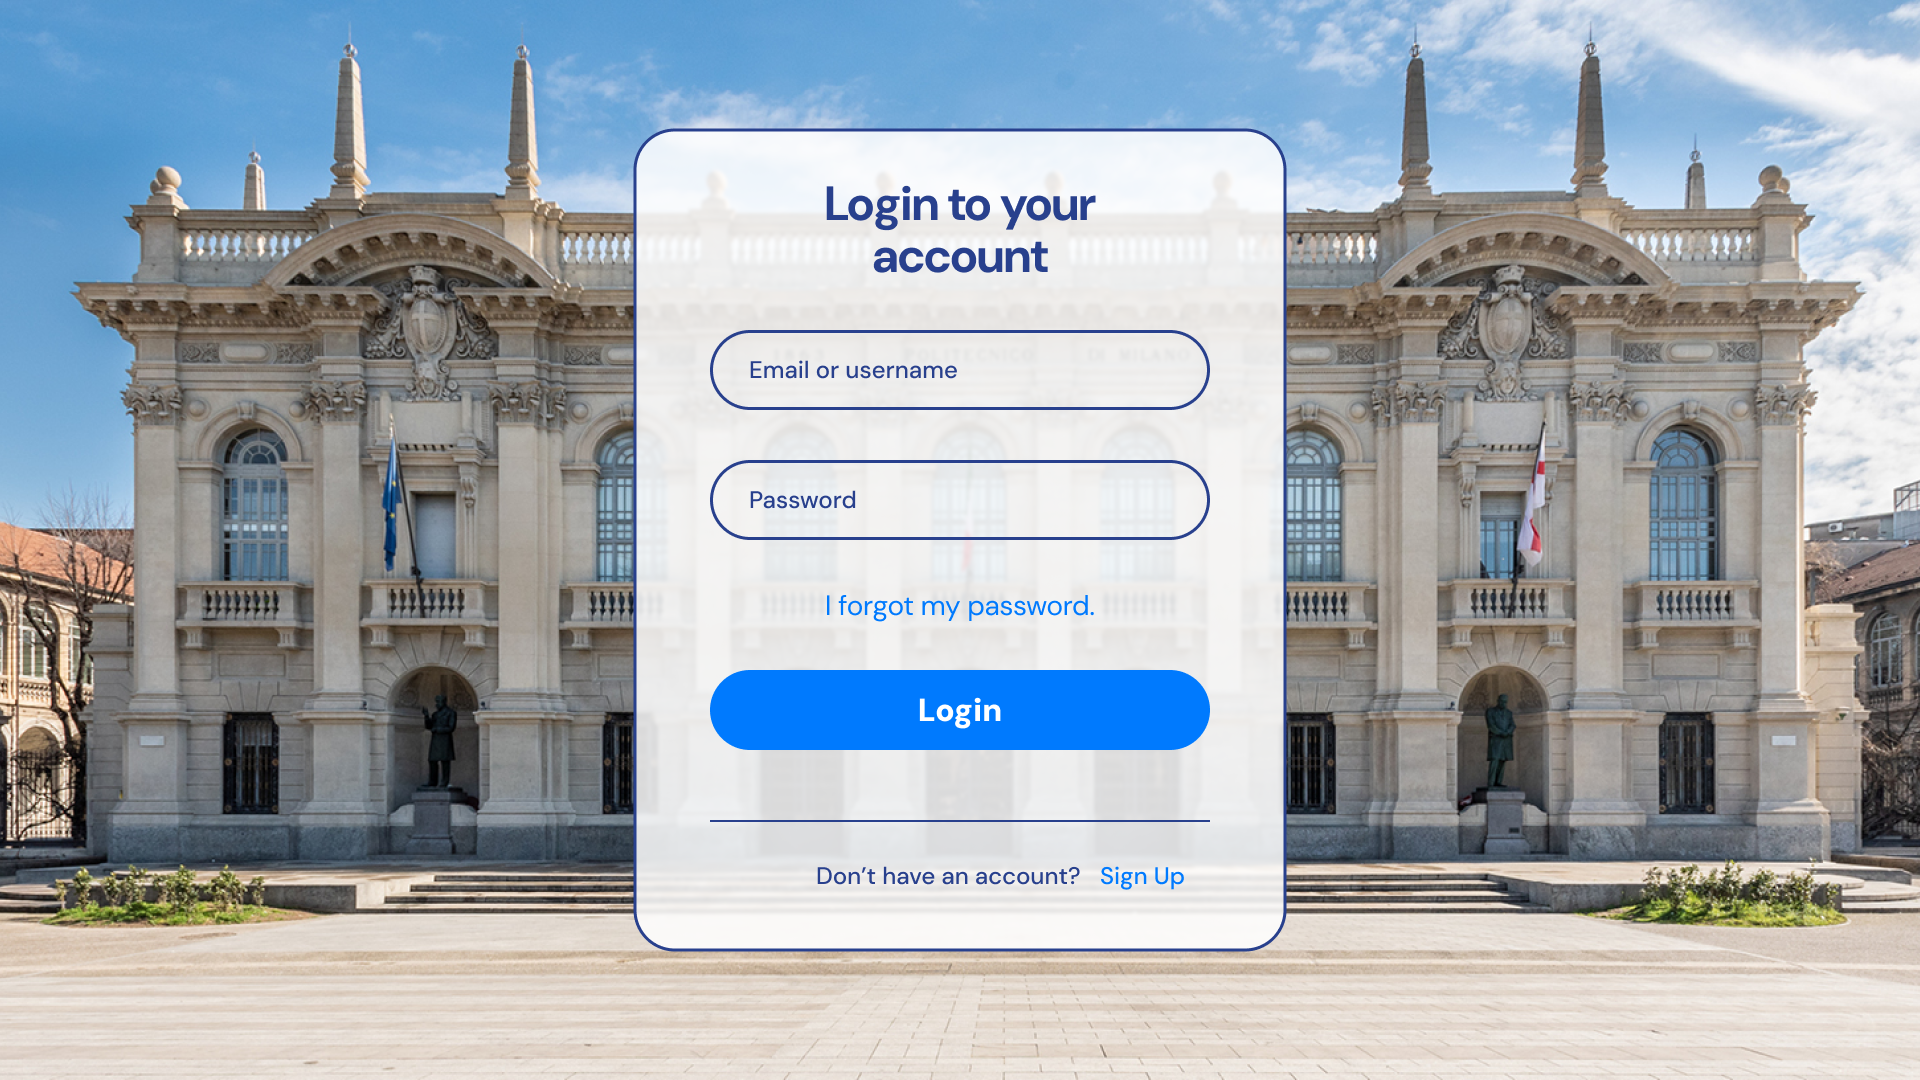
\includegraphics[width=0.98\textwidth]{Images/Login}
\caption{Login prototype page}\label{Login}
\end{figure}
\begin{figure}[H]
\centering
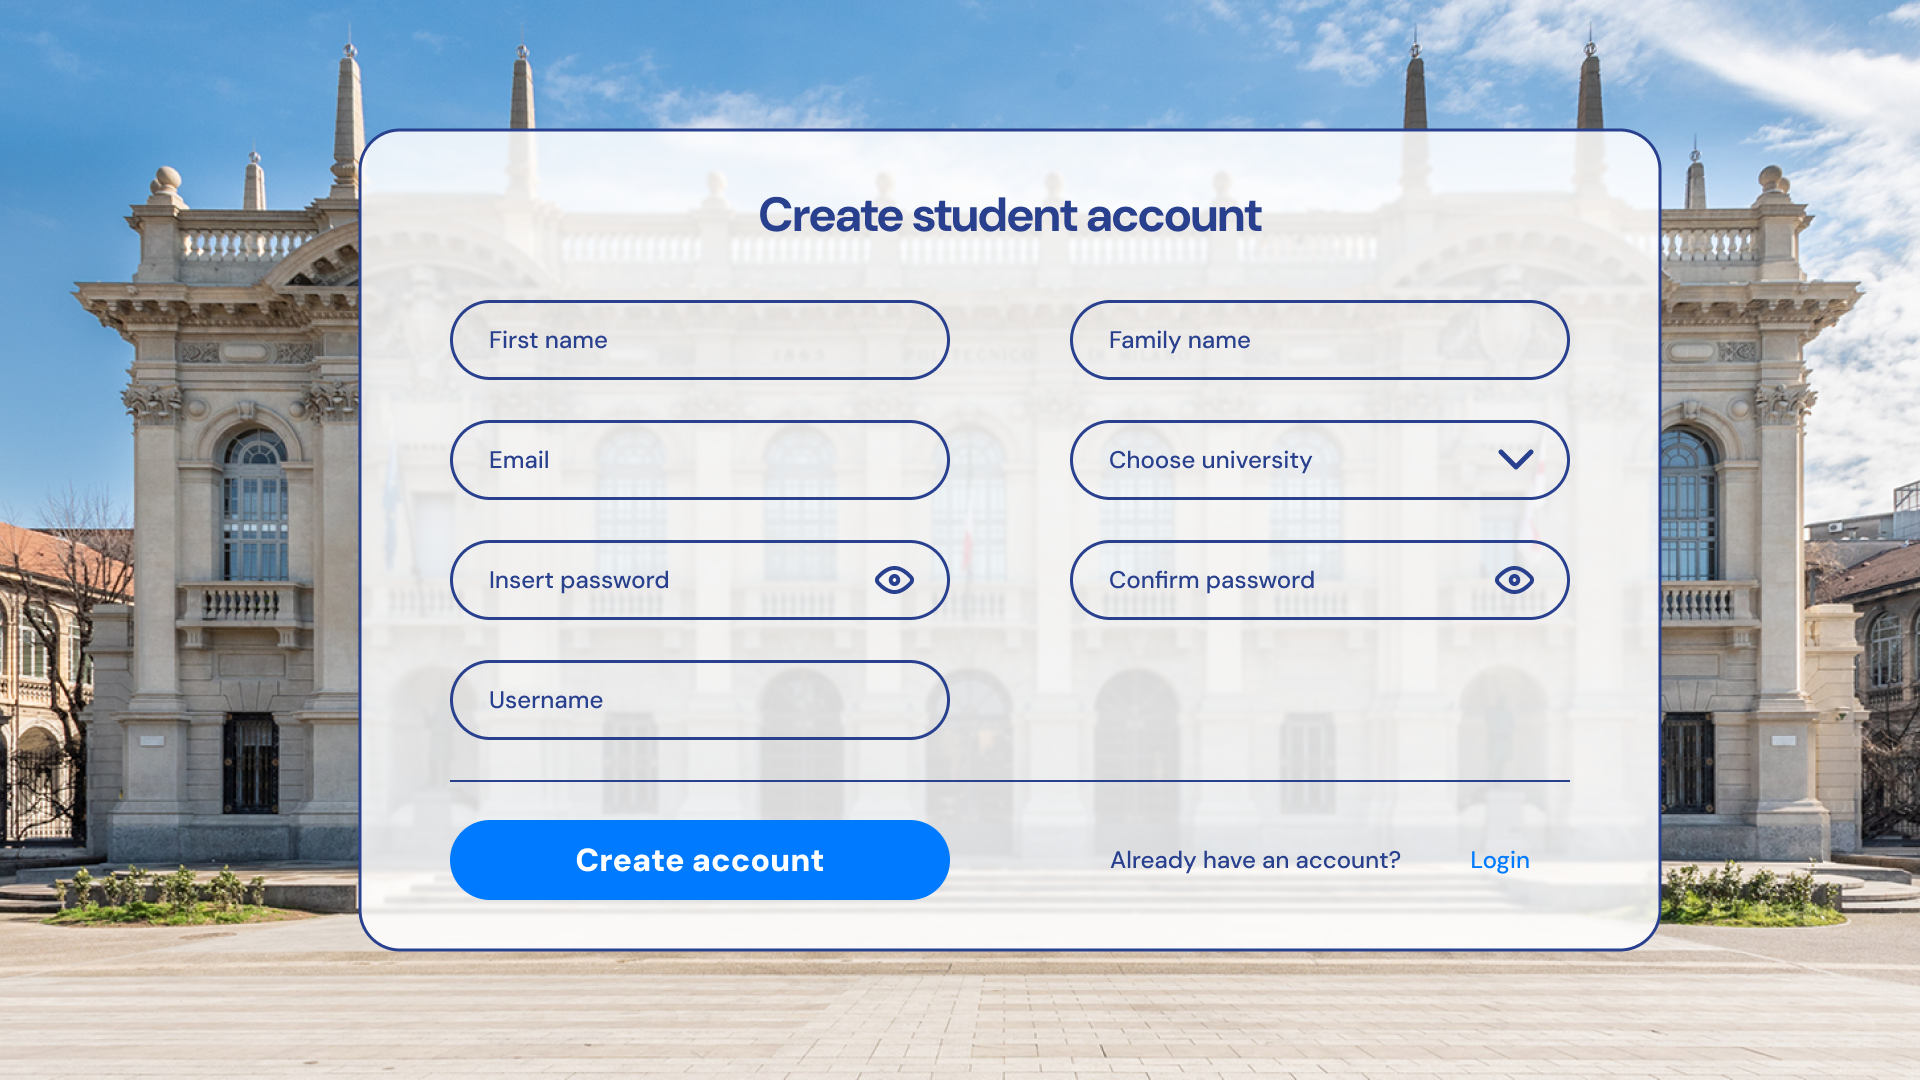
\includegraphics[width=0.98\textwidth]{Images/Sign Up}
\caption{Sign up prototype page}\label{Sign Up}
\end{figure}
\newpage
The picture [\ref{Login}] shows the prototype of the login page, allowing to either login by entering the correct credentials, create an account in case the user doesn't have one yet, or reset the password in case it was forgotten.\\
The picture [\ref{Sign Up}] shows the prototype of the sign up page for students, that allows students to create a new account by entering all the required information. In case the user already has an account there is a button that redirects to the login page. The case of a company creating an account is really similar to the one shown above with the simple difference that the user wont be required to choose a university.
\vspace{1\baselineskip} \\
\large{\textbf{Profile page}}
\begin{figure}[H]
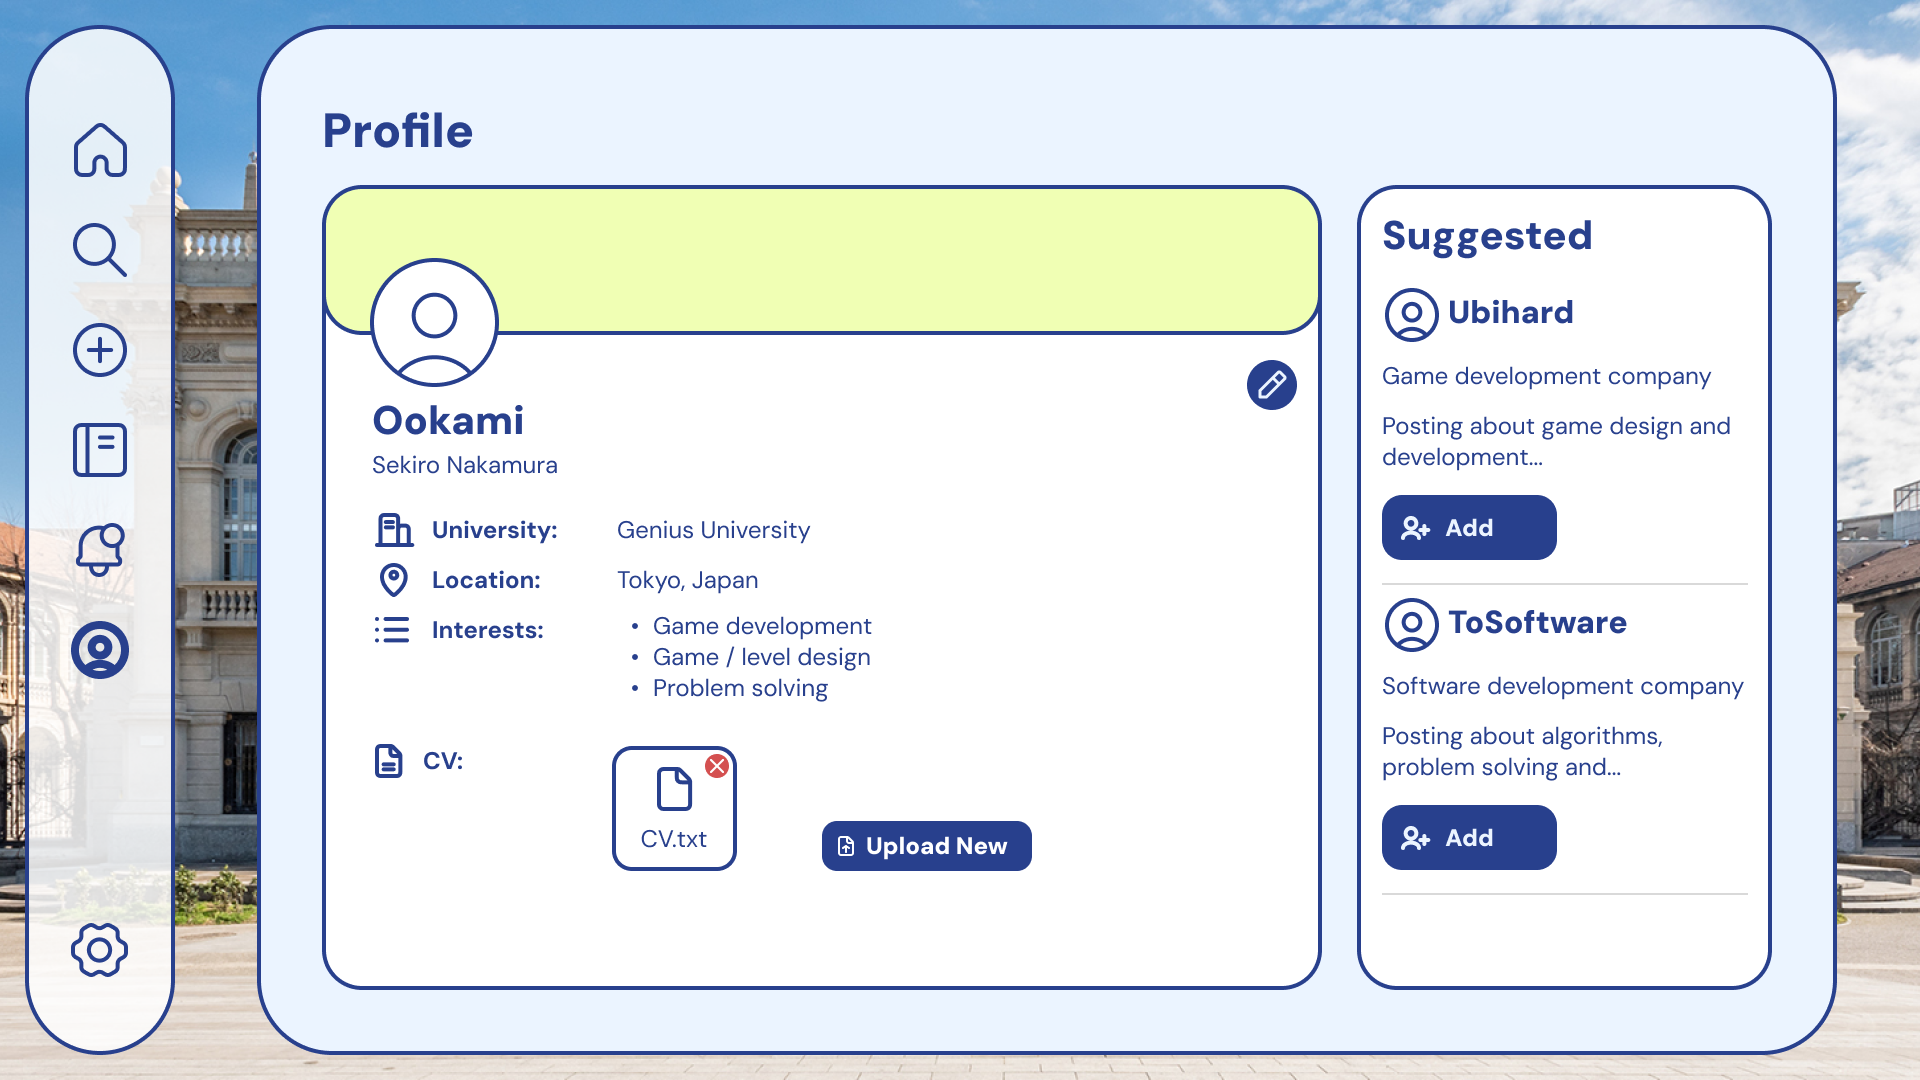
\includegraphics[width=\textwidth]{Images/Profile}
\caption{Student profile prototype page}\label{Student Profile}
\end{figure}
The picture [\ref{Student Profile}] shows the prototype of the profile page of a user logged in as a student. On the left, there is the section containing all the information provided by the user, and through the pencil button on the right, the user can modify the information. On the bottom there is the CV section. By clicking the file icon it opens the file allowing the user to check if the uploaded file is correct, otherwise the button on the right allows to upload a different file.\\
On the right side of the picture there is the "Suggested" area that show all the companies that might interest the user based on his interests.
\newpage
\large{\textbf{Notifications page}}
\begin{figure}[H]
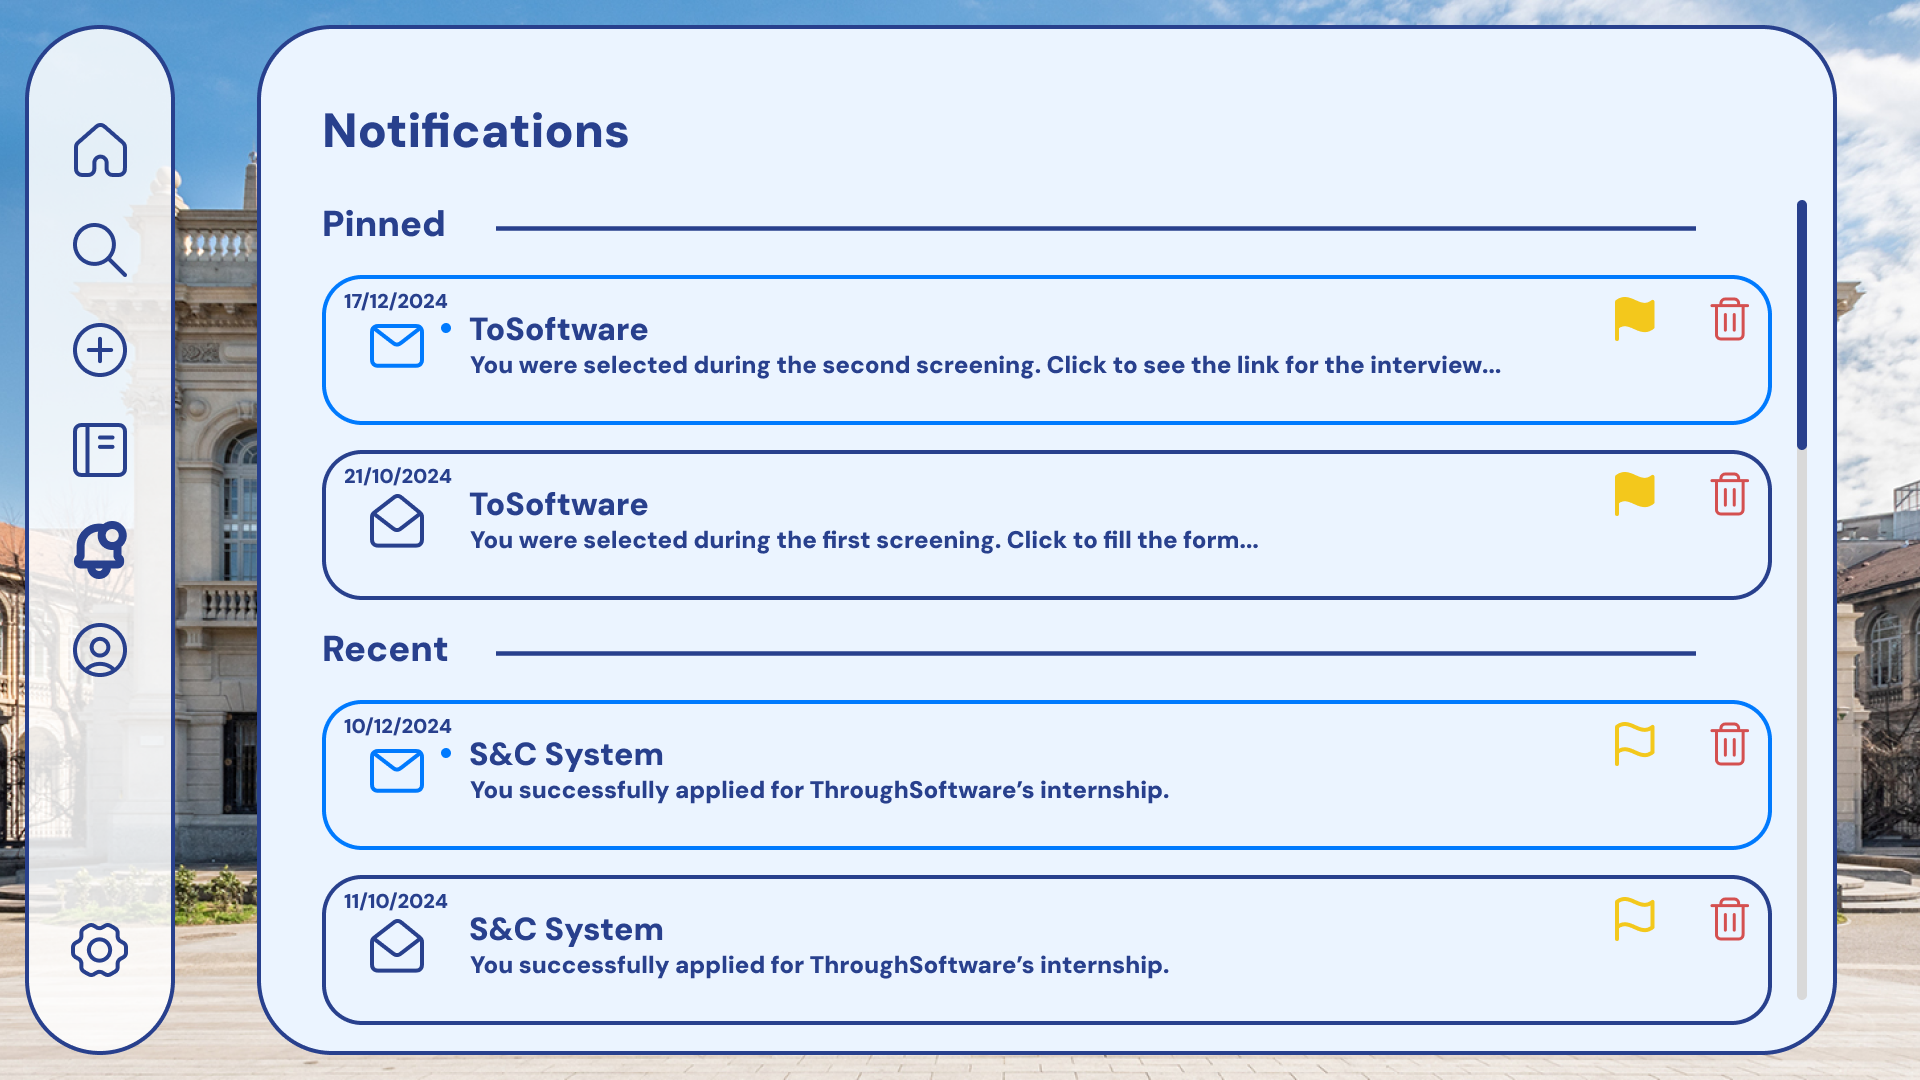
\includegraphics[width=\textwidth]{Images/Notifications}
\caption{Notifications prototype page}\label{Notifications}
\end{figure}
The picture [\ref{Notifications}] shows the prototype of the notifications page and is show to all three user categories. In general all notifications shown in the page render only a part of the whole message, and clicking on it allows the user to open a page that shows the whole text. In addition, notifications can be pinned to be always shown on top in their specific section by clicking on the yellow flag, or can be also permanently deleted by clicking on the trash can.
\newpage
\large{\textbf{Search page}}
\begin{figure}[H]
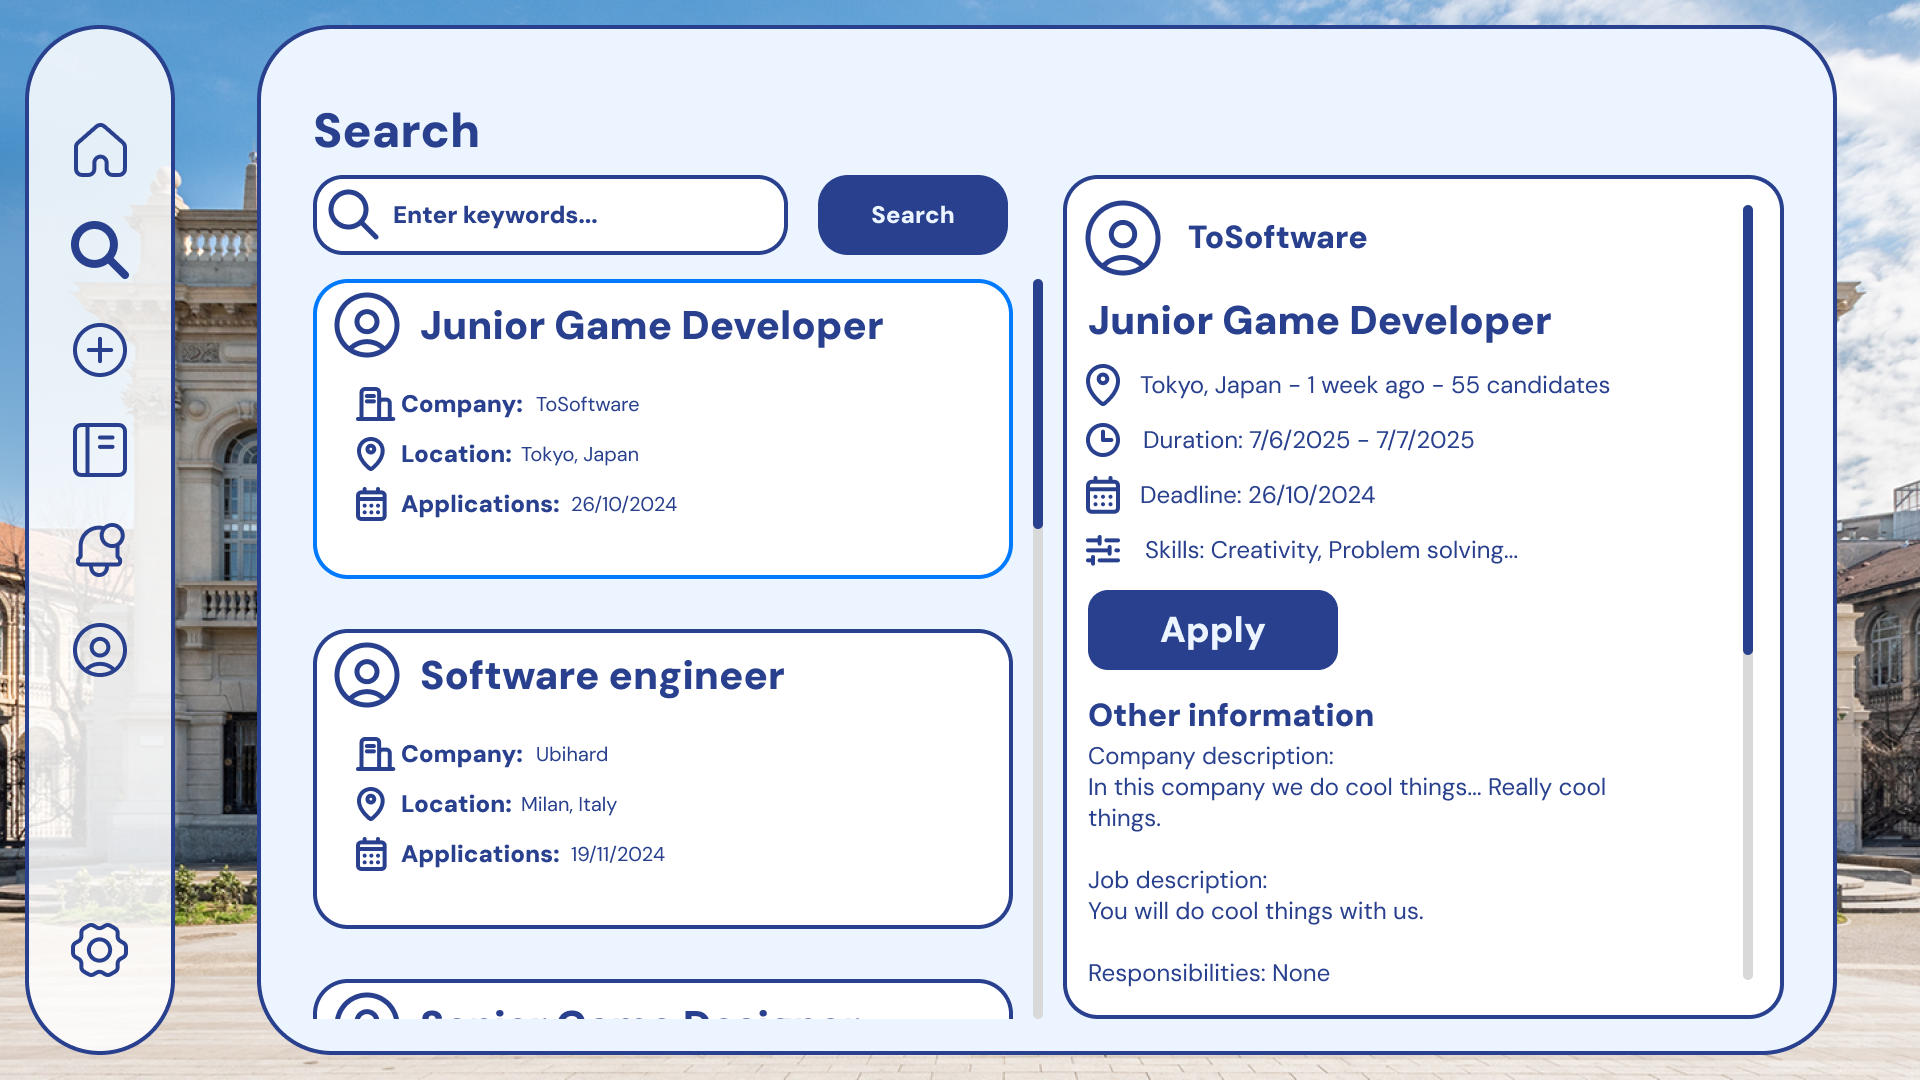
\includegraphics[width=\textwidth]{Images/Search}
\caption{Search prototype page}\label{Search}
\end{figure}
The picture [\ref{Search}] shows the prototype of the search page, that allow students to proactively search for internship by entering keywords in the search bar.\\
Right after searching the keywords the internship found are displayed on the left side and only show the basic details. By clicking on the desired internship, all the additional information entered by the company are displayed on the right side. Only when visualizing the details of an internship it is possible to apply for said offer through a dedicated button.
\newpage
\large{\textbf{Form creation page}}
\begin{figure}[H]
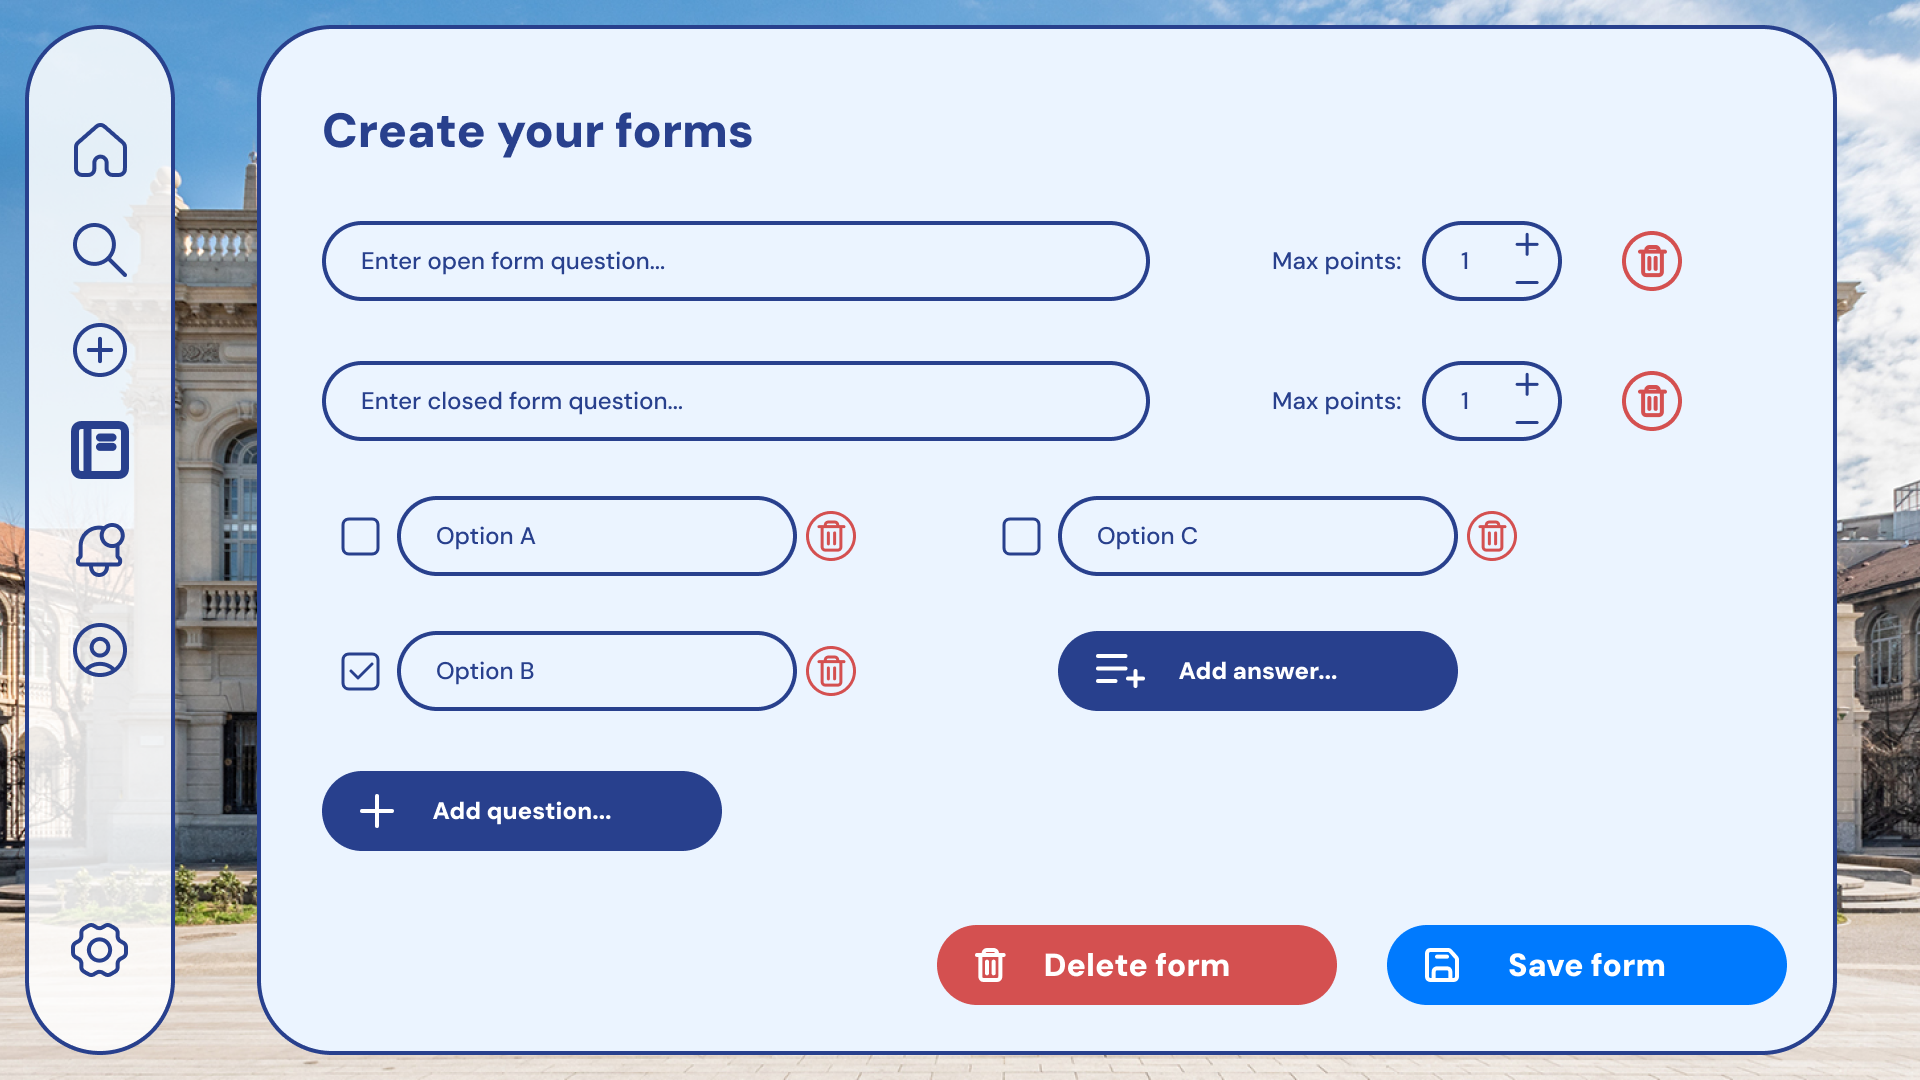
\includegraphics[width=\textwidth]{Images/Create form}
\caption{Form creation prototype page}\label{Form}
\end{figure}
The picture [\ref{Form}] shows the prototype of the form creation page that allows only companies to create custom forms for the candidates to fill during an application. In the form can be added two different types of questions: open and closed.\\
Open question only require the question text and the number of maximum point. \\
The closed ones not only require the question text and the maximum points like the open ones, but they also need the options the candidates have to choose from. Each option can be either deleted, marked as correct with the checkbox on the left, or can have its text changed. In addition the company can choose to add more options to the closed question with the \textit{"Add answer..."} button. \\
Lastly the company can decide to either add questions with the \textit{"Add question..."} button or delete them with the trash can icon on the right.\\
Once the form has been completed it can be saved or deleted by using the dedicated buttons.

\newpage

\large{\textbf{Home page}}
\begin{figure}[H]
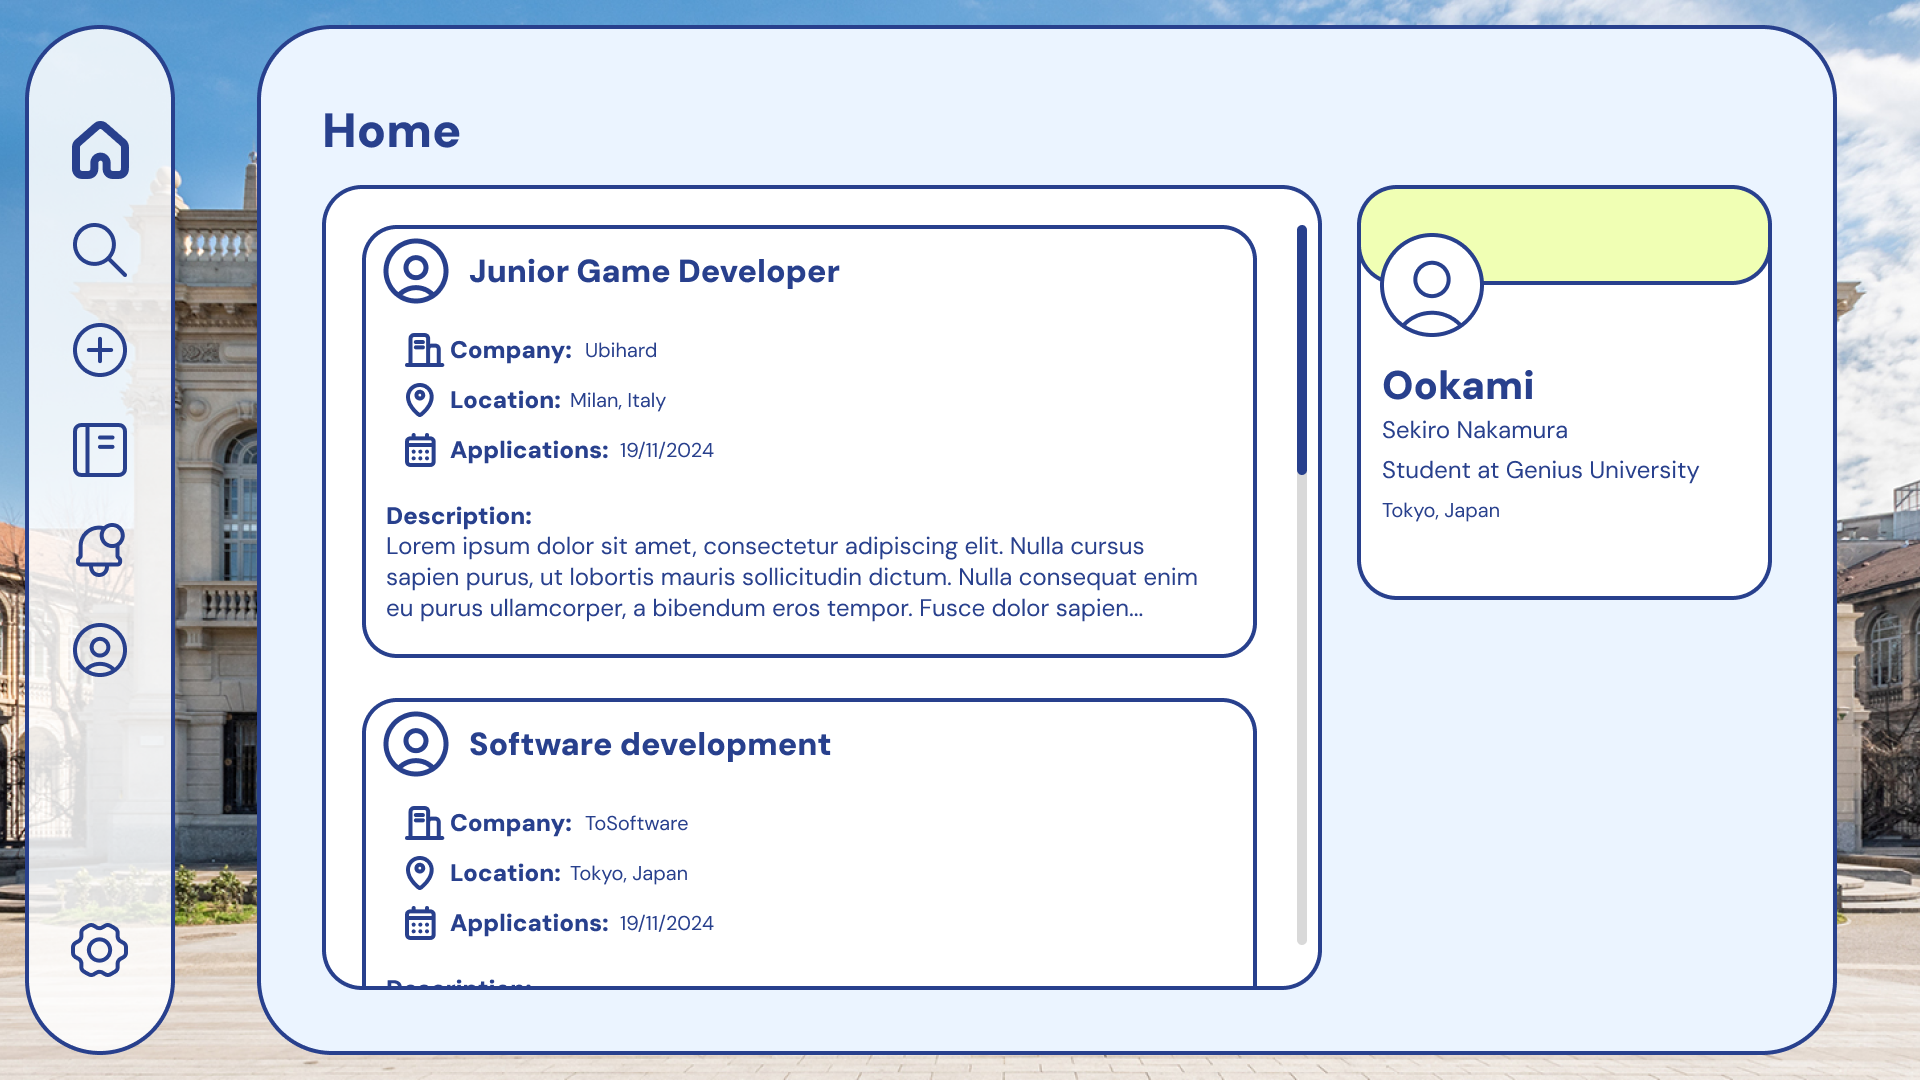
\includegraphics[width=\textwidth]{Images/Home}
\caption{Home prototype page}\label{Home}
\end{figure}
The picture [\ref{Home}] shows the prototype of the home page that allows students to see all the available internships posted by various companies.\\
The section on the left shows all the internships and by interacting with them the student can access a page that shows more details about the post and apply for the internship.\\
On the right there is a panel that shows the basic data regarding the user that is currently logged in.

\newpage

\large{\textbf{Internship creation page}}
\begin{figure}[H]
\includegraphics[width=\textwidth]{Images/Create internship}
\caption{Internship creation prototype page}\label{Create internship}
\end{figure}
The picture [\ref{Create internship}] shows the prototype of the page that allows companies to create and post about an internship.\\
In this page the company can add all the required information that allows the system to select the suitable students and notify them.

\newpage

\section{Requirement traceability}

\newpage

\section{Implementation, integration and test plan}

\newpage

\section{Effort spent}

\begin{itemize}

\item \textbf{Abdallah Alkhetiar}
\begin{table}[H]
\begin{tabular}{| >{\centering\arraybackslash}m{0.2\textwidth} || >{\centering\arraybackslash}m{0.2\textwidth} |}
\hline
\textbf{Chapter} & \textbf{Effort} \\
\hline
1 & 0 h \\
\hline
2 & 0 h \\
\hline
3 & 0 h \\
\hline
4 & 0 h \\
\hline
5 & 0 h \\
\hline
\end{tabular}
\end{table}

\vspace{1\baselineskip}

\item \textbf{Daniel Bonardi}
\begin{table}[H]
\begin{tabular}{| >{\centering\arraybackslash}m{0.2\textwidth} || >{\centering\arraybackslash}m{0.2\textwidth} |}
\hline
\textbf{Chapter} & \textbf{Effort} \\
\hline
1 & 0 h \\
\hline
2 & 0 h \\
\hline
3 & 0 h \\
\hline
4 & 0 h \\
\hline
5 & 0 h \\
\hline
\end{tabular}
\end{table}

\end{itemize}

\newpage

\section{References}
\textbf{N-tier architectures}\\
\href{https://dev.to/3bdelrahman/understanding-layers-tiers-and-n-tier-architecture-in-application-development-1hlb}{\textcolor{blue}{https://dev.to/3bdelrahman}}\\
\href{https://blog.nginx.org/blog/time-to-move-to-a-four-tier-application-architecture#:~:text=Forrester\%27s\%20Four‑Tier\%20Engagement\%20Platform,\%2C\%20aggregation\%2C\%20and\%20services\%20layers.}{\textcolor{blue}{https://blog.nginx.org/blog}}\\
\href{https://www.klipfolio.com/resources/data-stack/integration-layer}{\textcolor{blue}{https://www.klipfolio.com}}

\end{document}